
%   Copyright 2012 Comet Engineering, Patrick Haring & Christian Bürgi
%
%   Licensed under the Apache License, Version 2.0 (the "License");
%   you may not use this file except in compliance with the License.
%   You may obtain a copy of the License at
%
%       http://www.apache.org/licenses/LICENSE-2.0
%
%   Unless required by applicable law or agreed to in writing, software
%   distributed under the License is distributed on an "AS IS" BASIS,
%   WITHOUT WARRANTIES OR CONDITIONS OF ANY KIND, either express or implied.
%   See the License for the specific language governing permissions and
%   limitations under the License.

\documentclass[fontsize=12pt,
               paper=a4,
               twoside=false,
               parskip=half,
               ]{scrartcl}

% Load the packages
%   Copyright 2012 Comet Engineering, Patrick Haring & Christian Bürgi
%
%   Licensed under the Apache License, Version 2.0 (the "License");
%   you may not use this file except in compliance with the License.
%   You may obtain a copy of the License at
%
%       http://www.apache.org/licenses/LICENSE-2.0
%
%   Unless required by applicable law or agreed to in writing, software
%   distributed under the License is distributed on an "AS IS" BASIS,
%   WITHOUT WARRANTIES OR CONDITIONS OF ANY KIND, either express or implied.
%   See the License for the specific language governing permissions and
%   limitations under the License.

% Packages Template
% =================
% 
% Contains packages used for project documentation
% 
% @author burgc5
% 
% To use this simply enter: %   Copyright 2012 Comet Engineering, Patrick Haring & Christian Bürgi
%
%   Licensed under the Apache License, Version 2.0 (the "License");
%   you may not use this file except in compliance with the License.
%   You may obtain a copy of the License at
%
%       http://www.apache.org/licenses/LICENSE-2.0
%
%   Unless required by applicable law or agreed to in writing, software
%   distributed under the License is distributed on an "AS IS" BASIS,
%   WITHOUT WARRANTIES OR CONDITIONS OF ANY KIND, either express or implied.
%   See the License for the specific language governing permissions and
%   limitations under the License.

% Packages Template
% =================
% 
% Contains packages used for project documentation
% 
% @author burgc5
% 
% To use this simply enter: %   Copyright 2012 Comet Engineering, Patrick Haring & Christian Bürgi
%
%   Licensed under the Apache License, Version 2.0 (the "License");
%   you may not use this file except in compliance with the License.
%   You may obtain a copy of the License at
%
%       http://www.apache.org/licenses/LICENSE-2.0
%
%   Unless required by applicable law or agreed to in writing, software
%   distributed under the License is distributed on an "AS IS" BASIS,
%   WITHOUT WARRANTIES OR CONDITIONS OF ANY KIND, either express or implied.
%   See the License for the specific language governing permissions and
%   limitations under the License.

% Packages Template
% =================
% 
% Contains packages used for project documentation
% 
% @author burgc5
% 
% To use this simply enter: \input{./packages.tex}

\usepackage[utf8]{inputenc}
\usepackage[T1]{fontenc}

% Set font to latin modern
\usepackage{lmodern}

\usepackage[pdftex]{graphicx}
\usepackage{epstopdf}

% Create links in pdf documents
\usepackage[colorlinks,pdfpagelabels,pdfstartview=FitH,bookmarksopen=true,bookmarksnumbered=true,linkcolor=black,plainpages=false,hypertexnames=false,citecolor=black] {hyperref}
\hypersetup{
    colorlinks,%
    citecolor=black,%
    filecolor=black,%
    linkcolor=black,%
    urlcolor=black
}
\urlstyle{same}

% Use \enquote{} to create quotation marks
\usepackage{csquotes}

% Create professional tables with booktabs
% @see http://en.wikibooks.org/wiki/LaTeX/Tables#Professional_tables
\usepackage{booktabs}

% Customizable enumerates/itemizes
\usepackage{enumitem}

% git meta information
\usepackage{gitinfo}


\usepackage[utf8]{inputenc}
\usepackage[T1]{fontenc}

% Set font to latin modern
\usepackage{lmodern}

\usepackage[pdftex]{graphicx}
\usepackage{epstopdf}

% Create links in pdf documents
\usepackage[colorlinks,pdfpagelabels,pdfstartview=FitH,bookmarksopen=true,bookmarksnumbered=true,linkcolor=black,plainpages=false,hypertexnames=false,citecolor=black] {hyperref}
\hypersetup{
    colorlinks,%
    citecolor=black,%
    filecolor=black,%
    linkcolor=black,%
    urlcolor=black
}
\urlstyle{same}

% Use \enquote{} to create quotation marks
\usepackage{csquotes}

% Create professional tables with booktabs
% @see http://en.wikibooks.org/wiki/LaTeX/Tables#Professional_tables
\usepackage{booktabs}

% Customizable enumerates/itemizes
\usepackage{enumitem}

% git meta information
\usepackage{gitinfo}


\usepackage[utf8]{inputenc}
\usepackage[T1]{fontenc}

% Set font to latin modern
\usepackage{lmodern}

\usepackage[pdftex]{graphicx}
\usepackage{epstopdf}

% Create links in pdf documents
\usepackage[colorlinks,pdfpagelabels,pdfstartview=FitH,bookmarksopen=true,bookmarksnumbered=true,linkcolor=black,plainpages=false,hypertexnames=false,citecolor=black] {hyperref}
\hypersetup{
    colorlinks,%
    citecolor=black,%
    filecolor=black,%
    linkcolor=black,%
    urlcolor=black
}
\urlstyle{same}

% Use \enquote{} to create quotation marks
\usepackage{csquotes}

% Create professional tables with booktabs
% @see http://en.wikibooks.org/wiki/LaTeX/Tables#Professional_tables
\usepackage{booktabs}

% Customizable enumerates/itemizes
\usepackage{enumitem}

% git meta information
\usepackage{gitinfo}


\begin{document}

% Document title for title.tex
\newcommand{\doctitle}{Supplementary Specification}
% Titlepage Template
% ==================
% 
% @author burgc5
% 
% To use this simply enter: % Titlepage Template
% ==================
% 
% @author burgc5
% 
% To use this simply enter: % Titlepage Template
% ==================
% 
% @author burgc5
% 
% To use this simply enter: \input{./title.tex}
% 
% You have to define the commands '\doctitle' and '\docrevision' to give the 
% document a title and a revision on its titlepage.
% Do this with the following command:
% \newcommand{\doctitle}{Document title goes here}
%
% SVN:
% ----
% You also have to define the variables:
% \SVN $Date$
% \SVN $Revision$
%
% As executing the following command on the file:
% > svn propset svn:keywords "Date Revision" filename.tex
% 
% This titlepage needs:
% \usepackage[pdftex]{graphicx}
% \usepackage{svn}
%

\begin{titlepage}

\begin{center}

% Team-logo

\includegraphics[width=0.35\textwidth]{./comet-logo.eps}\\[2.5cm]    

% Project title
\textsc{\Large Comet Pinball}\\[2cm]

% Document title
{ \huge \bfseries \doctitle{}}\\[3cm]

% Members/Client
\begin{minipage}{0.45\textwidth}
\begin{flushleft} \large
\emph{Team Members:}\\
Patrick \textsc{Haring}\\
Christian \textsc{Bürgi}
\end{flushleft}
\end{minipage}
\begin{minipage}{0.45\textwidth}
\begin{flushright} \large
\emph{Client:} \\
Jean-Pierre \textsc{Caillot}\\
~
\end{flushright}
\end{minipage}

\vfill

{\large 
Revision hash: \gitAbbrevHash \\[0.2cm]
Commit time: \gitCommitterIsoDate \\[0.2cm]
{\footnotesize \itshape \url{https://github.com/boskoop/comet-pinball/}}}

\end{center}

\end{titlepage}
% 
% You have to define the commands '\doctitle' and '\docrevision' to give the 
% document a title and a revision on its titlepage.
% Do this with the following command:
% \newcommand{\doctitle}{Document title goes here}
%
% SVN:
% ----
% You also have to define the variables:
% \SVN $Date$
% \SVN $Revision$
%
% As executing the following command on the file:
% > svn propset svn:keywords "Date Revision" filename.tex
% 
% This titlepage needs:
% \usepackage[pdftex]{graphicx}
% \usepackage{svn}
%

\begin{titlepage}

\begin{center}

% Team-logo

\includegraphics[width=0.35\textwidth]{./comet-logo.eps}\\[2.5cm]    

% Project title
\textsc{\Large Comet Pinball}\\[2cm]

% Document title
{ \huge \bfseries \doctitle{}}\\[3cm]

% Members/Client
\begin{minipage}{0.45\textwidth}
\begin{flushleft} \large
\emph{Team Members:}\\
Patrick \textsc{Haring}\\
Christian \textsc{Bürgi}
\end{flushleft}
\end{minipage}
\begin{minipage}{0.45\textwidth}
\begin{flushright} \large
\emph{Client:} \\
Jean-Pierre \textsc{Caillot}\\
~
\end{flushright}
\end{minipage}

\vfill

{\large 
Revision hash: \gitAbbrevHash \\[0.2cm]
Commit time: \gitCommitterIsoDate \\[0.2cm]
{\footnotesize \itshape \url{https://github.com/boskoop/comet-pinball/}}}

\end{center}

\end{titlepage}
% 
% You have to define the commands '\doctitle' and '\docrevision' to give the 
% document a title and a revision on its titlepage.
% Do this with the following command:
% \newcommand{\doctitle}{Document title goes here}
%
% SVN:
% ----
% You also have to define the variables:
% \SVN $Date$
% \SVN $Revision$
%
% As executing the following command on the file:
% > svn propset svn:keywords "Date Revision" filename.tex
% 
% This titlepage needs:
% \usepackage[pdftex]{graphicx}
% \usepackage{svn}
%

\begin{titlepage}

\begin{center}

% Team-logo

\includegraphics[width=0.35\textwidth]{./comet-logo.eps}\\[2.5cm]    

% Project title
\textsc{\Large Comet Pinball}\\[2cm]

% Document title
{ \huge \bfseries \doctitle{}}\\[3cm]

% Members/Client
\begin{minipage}{0.45\textwidth}
\begin{flushleft} \large
\emph{Team Members:}\\
Patrick \textsc{Haring}\\
Christian \textsc{Bürgi}
\end{flushleft}
\end{minipage}
\begin{minipage}{0.45\textwidth}
\begin{flushright} \large
\emph{Client:} \\
Jean-Pierre \textsc{Caillot}\\
~
\end{flushright}
\end{minipage}

\vfill

{\large 
Revision hash: \gitAbbrevHash \\[0.2cm]
Commit time: \gitCommitterIsoDate \\[0.2cm]
{\footnotesize \itshape \url{https://github.com/boskoop/comet-pinball/}}}

\end{center}

\end{titlepage}

\tableofcontents

\section{Introduction}
In Unified Process methodology, the document \emph{Supplementary Specification} contains all the non-functional requirements. (The functional requirements are specified with \emph{Use Cases}.)

Some additional non-functional requirements are currently covered in the Vision Document.

\section{Non-functional requirements}

\subsection{Usability}
\begin{itemize}
	\item[U1] Avoid colors associated with common forms of color blindness.
	\item[U2] The interface should be as intuitive as possible.
	\item[U3] The key mapping should be customizable.
\end{itemize}

\subsection{Reliability}
\begin{itemize}
	\item[R1] When the application is closed unexpectedly the data integrity should not be harmed.
\end{itemize}

\subsection{Performance}
\begin{itemize}
	\item[P1] The application should run on entry-level computer with over 30 frames per second.
\end{itemize}

\subsection{Supportability}
\begin{itemize}
	\item[S1] The system has to run on Unix/GNU-Linux as well as on Microsoft Windows and Mac OS X.	
\end{itemize}

\section{Technical specifications}
\begin{itemize}
	\item[T1] Java 6 is used.
	\item[T2] The cross-platform game development library libgdx is used. 
\end{itemize}

\subsection{Libraries}
The following libraries have been used in the project:

\begin{tabular}{| l | l | l |}
	\hline
	\textbf{Name} & \textbf{Version} & \textbf{Link} \\ \hline
	Apache Commons Lang & 3.1 & \url{http://commons.apache.org/lang/} \\ \hline
	Apache Commons IO & 2.4 & \url{http://commons.apache.org/io/} \\ \hline
	JUnit & 4.10 & \url{http://junit.sourceforge.net} \\ \hline
	Libgdx & 0.9.7 & \url{http://libgdx.badlogicgames.com} \\ \hline
	Logback & 1.0.9 & \url{http://logback.qos.ch} \\ \hline
	Mockito & 1.9.5 & \url{http://code.google.com/p/mockito/} \\ \hline
	PicoContainer & 2.13.6 & \url{http://picocontainer.codehaus.org} \\ \hline
	SLF4J & 1.7.2 & \url{http://slf4j.org} \\ \hline
	Sysout-over-slf4j & 1.0.2 & \url{http://projects.lidalia.org.uk/sysout-over-slf4j/} \\ \hline
	Universal Tween Engine & 6.3.3 & \url{http://www.aurelienribon.com} \\ \hline
\end{tabular}

\section{Tools}
\begin{tabular}{| l | l | l | l |}
	\hline
	\textbf{Name} & \textbf{Version} & \textbf{Usage} & \textbf{Link} \\ \hline
	Apache Maven & 3.0.x & Build automation & \url{http://maven.apache.org} \\ \hline
	Artifactory & 2.6.4 & Repository manager & \url{http://www.jfrog.com} \\ \hline
	Astah community & 6.6.4 & UML diagrams & \url{http://www.astah.net} \\ \hline
	Eclipse & 4.2 & Java development & \url{http://www.eclipse.org} \\ \hline
	Git & 1.8 & Revision control & \url{http://git-scm.com} \\ \hline
	Github & - & Collaboration & \url{http://www.github.com} \\ \hline
	Jenkins & 1.499 & Build Server & \url{http://jenkins-ci.org} \\ \hline
	LaTeX & TeX Live 2012 & Documentation & \url{http://www.tug.org/texlive/} \\ \hline
	Redmine & 2.1 & Project management & \url{http://www.redmine.org} \\ \hline
\end{tabular}

\section{Development environment}

In order to create a stable build process without integration problems, we use a Jenkins build server. The build is done using Apache Maven. The source is managed using git version control system. Figure~\ref{fig:build_environment} explains the setup we used for the process.

\begin{figure}[h!]
	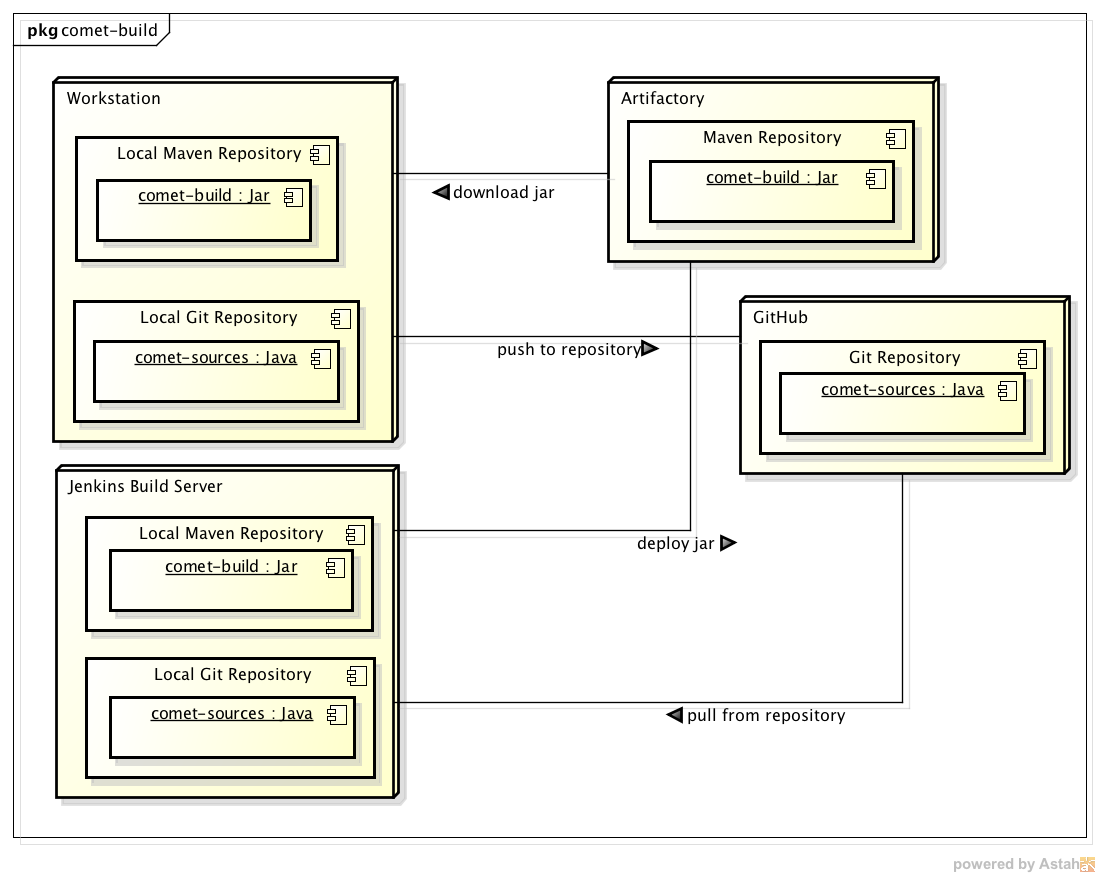
\includegraphics[width=15.5cm]{./img/comet-build.png}
	\caption[Comet build environment]{Comet build environment}
	\label{fig:build_environment}
\end{figure}

The developer writes his code on his workstation and checks it into the local git repository. The code is committed and pushed into the remote Github repository, where it is made available to every developer in the team. The Jenkins build server pulls on his scheduled builds the current version of the codebase into his local repository and builds. Maven installs the artefact into its build-server-local repository and deploys it to the Artifactory. The developers update their local Maven repository by downloading the jars from Artifactory.

\subsection{Github configuration}

The source repository is hosted at the following location: \url{https://github.com/boskoop/comet-pinball/}, a standard git installation is required to access the source.

\subsection{Maven configuration}

The developers need the following Maven configuration file in order to connect their Maven installation to the Artifactory server.

\begin{lstlisting}[language=xml,label=lst:settings_xml,caption={settings.xml}]
<?xml version="1.0" encoding="UTF-8"?>
<settings xmlns="http://maven.apache.org/SETTINGS/1.0.0" 
	xmlns:xsi="http://www.w3.org/2001/XMLSchema-instance" 
	xsi:schemaLocation="http://maven.apache.org/SETTINGS/1.0.0 http://maven.apache.org/xsd/settings-1.0.0.xsd">
	<pluginGroups>
	</pluginGroups>
	<proxies>
	</proxies>
	<servers>
		<server>
			<username><!-- username --></username>
			<password><!-- password --></password>
			<id>comet-artifactory</id>
		</server>
	</servers>
	<mirrors>
		<mirror>
			<mirrorOf>*</mirrorOf>
			<name>repo</name>
			<url>http://ci.m02.ch/artifactory/repo</url>
			<id>repo</id>
		</mirror>
	</mirrors>
	<profiles>
		<profile>
			<repositories>
				<repository>
					<snapshots>
						<enabled>false</enabled>
					</snapshots>
					<id>central</id>
					<name>libs-release</name>
					<url>http://ci.m02.ch/artifactory/libs-release</url>
				</repository>
				<repository>
					<snapshots />
					<id>snapshots</id>
					<name>libs-snapshot</name>
					<url>http://ci.m02.ch/artifactory/libs-snapshot</url>
				</repository>
			</repositories>
			<pluginRepositories>
				<pluginRepository>
					<snapshots>
						<enabled>false</enabled>
					</snapshots>
					<id>central</id>
					<name>plugins-release</name>
					<url>http://ci.m02.ch/artifactory/plugins-release</url>
				</pluginRepository>
				<pluginRepository>
					<snapshots />
					<id>snapshots</id>
					<name>plugins-snapshot</name>
					<url>http://ci.m02.ch/artifactory/plugins-snapshot</url>
				</pluginRepository>
			</pluginRepositories>
			<id>artifactory</id>
		</profile>
	</profiles>
	<activeProfiles>
		<activeProfile>artifactory</activeProfile>
	</activeProfiles>
</settings>
\end{lstlisting}





\end{document}
